\documentclass[DIN, pagenumber=false, fontsize=11pt, parskip=half]{scrartcl}

\usepackage{ngerman}
\usepackage[utf8]{inputenc}
\usepackage[T1]{fontenc}
\usepackage{textcomp}
\usepackage{amsmath}
\usepackage{amsfonts}
\usepackage{tikz}

% for matlab code
% bw = blackwhite - optimized for print, otherwise source is colored
\usepackage[framed,numbered,bw]{styles/exercise}
\usepackage{hyperref}

% for other code
%\usepackage{listings}

\setlength{\parindent}{0em}

% set section in CM
\setkomafont{section}{\normalfont\bfseries\Large}

\newcommand{\mytitle}[1]{{\noindent\Large\textbf{#1}}}
\newcommand{\mysection}[1]{\textbf{\section*{#1}}}
\newcommand{\mysubsection}[2]{\romannumeral #1) #2}


%===================================
\begin{document}

\noindent\textbf{Very Deep Learning} \hfill \textbf{Technische Universität Kaiserslautern} \\
WS 2022/23 \hfill Dr. Muhammad Zeshan Afzal \\

\mytitle{Exercise 4 - Language Models and Attention}

\textbf{Deadline: 23.01.2023 \hfill Total Marks: 30}


\section*{Submission}

\begin{itemize}
    \item Submissions through OLAT. Only one group member needs to submit it.
    \item Your submission should contain a PDF with the solutions to the exercise questions (and a python notebook file) zipped together in a single file.
    \item Include the group number along with the names and matriculation numbers of all group members on the PDF.
    \item For the Jupyter notebook, please save them with the outputs of your code displayed.
\end{itemize}

%===================================
\mysection{4.1. Language Models\hfill[2 + 2 + 2 + 2 = 8]}

Consider a vocabulary $\mathcal{V} = \{A, B, C\}$ and sequences of length $T = 10$. \\Assume $p(\mathbf{x}) = \prod_{t=1}^T p(x_t)$ with $p(x_t=A) = 0.2$, $p(x_t=B)=0.5$, and $p(x_t=C)=0.3$ for both the model and data distributions.

\mysubsection{1}{Calculate the amount of information (in $bits$) needed to predict the next character in a sequence with a simple (unigram) model.}

\mysubsection{2}{Calculate the perplexity $\mathrm{Perplexity}(p_{data}, p_{model})$} for the same model. Remark on how certain the model is about which letter to predict next.

\mysubsection{3}{Let us now assume that the model disribution is the same as before, but the data distribution is $p(x_t = A) = 1$ now. Calculate the perplexity again. What does this new perplexity tell you about the model?}

\mysubsection{4}{How many bits we need now to encode any possible outcome of $p_{data}$ using code optimized for $p_{model}$?}


%===================================
\mysection{4.2. Beam Search \hfill[2+5+2=9]}

Let $y = \{yes, ok, $ </s> $\}$ be a vocabulary where </s> is the end-of-string character. The following figure shows a search tree for generating the target string $T=t_1,t_2,\ldots$ from this vocabulary. Each node represents the conditional probability $p(t_n | t_1, ..., t_{n-1}, \mathbf{source})$, where $\mathbf{source}$ is the context variable.

\begin{figure}[h]
    \centering
    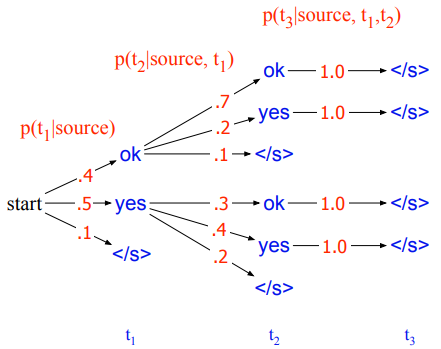
\includegraphics[width=0.6\linewidth]{img/4.2.png}
\end{figure}

\mysubsection{1}{What will be the generated target string in this case with the greedy search algorithm?}

\mysubsection{2}{Execute the beam search algorithm with the beam size $k=2$. What is the target string generated in this case? Compute all intermediate probabilities.}

\mysubsection{3}{Did the two search algorithms yield the same result? What is the benefit of using beam search over the greedy approach?}

%===================================
\mysection{4.3. Transformers and Attention \hfill[3+5+5=13]}

Given \begin{equation*}
X = \begin{bmatrix}
4 & 0 & 2 & 1 \\
0 & 1 & 1 & 2 \\
1 & 0 & 1 & 0
\end{bmatrix}, W_Q = \begin{bmatrix}
0 & 0 & 1 \\
0 & 1 & 0 \\
0 & 1 & 1 \\
1 & 0 & 0
\end{bmatrix}, W_K = \begin{bmatrix}
1 & 0 & 1 \\
1 & 1 & 0 \\
1 & 1 & 1 \\
0 & 0 & 1
\end{bmatrix}, W_V = \begin{bmatrix}
0 & 0 & 2 \\
3 & 0 & 0 \\
1 & 5 & 0 \\
0 & 1 & 0
\end{bmatrix}
\end{equation*} where $X$ is the input, and $W_Q, W_K,$ and $W_V$ are the weights for query, key and value respectively.

\mysubsection{1}{Explain the intuition behind the query, key and value in the attention mechanism.}

\mysubsection{2}{Compute self-attention for $X$ showing all the intermediate steps.}

\mysubsection{3}{Repeat the same steps you performed in part (ii) using simple PyTorch operations and verify that you get the same answers as in part (ii). Use the provided notebook \texttt{Task\_4.3.ipynb} for this task.}

\textbf{Good luck!}

\end{document}